\section{Conclusioni}
        Possiamo concludere che, a meno di un errore del 2-3\%, la misura della carica di un elettrone sia eseguibile tramite la metodologia da noi utilizzata.\\
        Dobbiamo considerare che la misura universalmente oggi accettata è frutto di molte più misurazioni di quelle prese dal nostro gruppo, con strumenti più raffinati e precisi.\\
        Tramite un'analisi statistica più consistente ed un più accurato rigetto dei dati abbiamo ottenuto che la carica elettrica dell'elettrone ha un valore:
        $$q_{e^-} = \left(-1.607\pm0.012\right)\cdot10^{-19}~\mathrm{C}$$
        Calcolando la discrepanza standardizzata del dato sperimentale rispetto al valore atteso, si ottiene che la carica dell'elettrone sperimentalmente ha un livello di confidenza pari a $0.43\sigma$ e una compatibilità del $92.80\%$ con la misura universalmente accettata.\\
        Dobbiamo anche ammettere di aver ottenuto una così grande compatibilità a causa della qualità delle nostre misurazioni, che ci hanno portato a ottenere un errore del $7.4\%$ sulla misura finale.\\
        Consideriamo tale errore accettabile al fine di un'esperienza di laboratorio didattica, ma non si tratta sicuramente di una misurazione estremamente accurata dal punto di vista sperimentale.
        \subsection{Grafico comparativo, carica effettiva/carica misurata}
\begin{figure}[H]
    \centering
    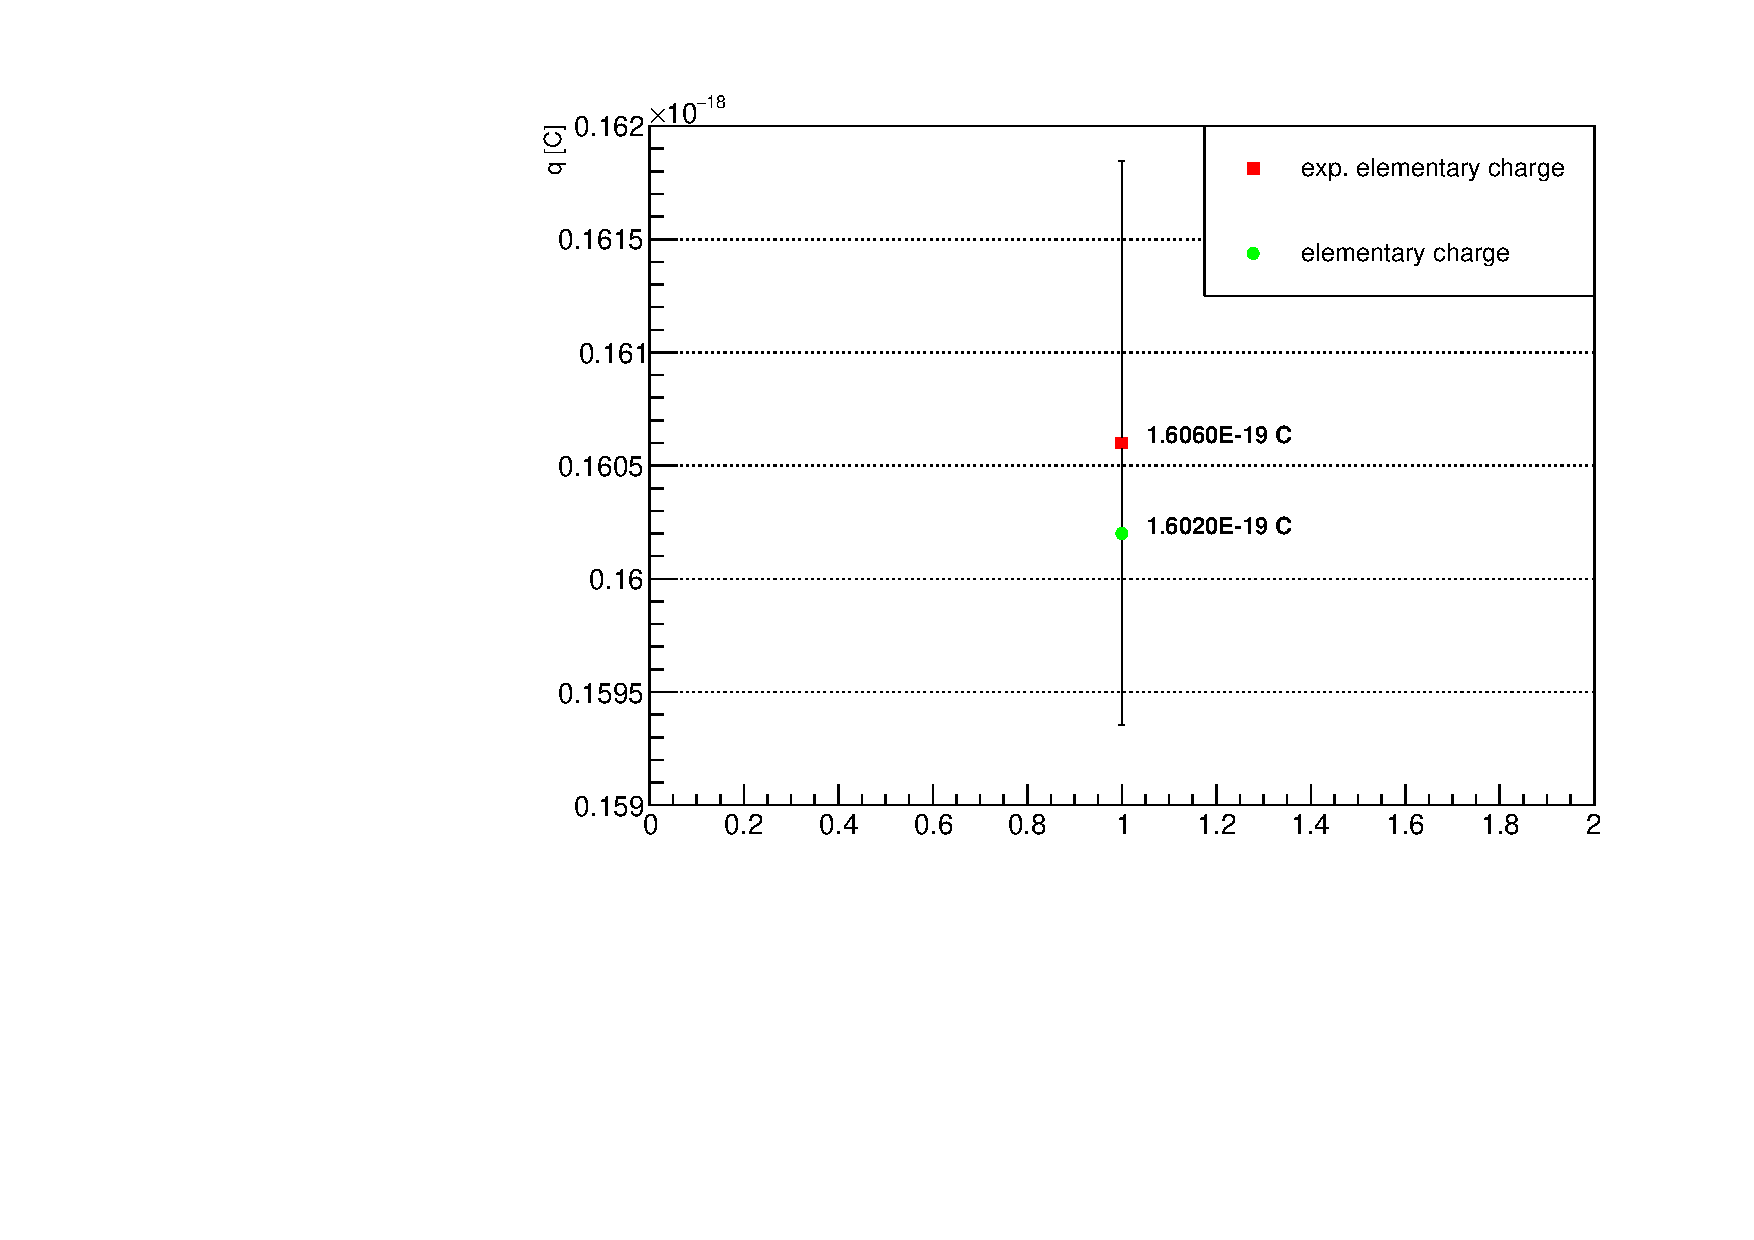
\includegraphics[width=\textwidth,height=\textheight,keepaspectratio]{graph2.pdf}
    \caption{Grafico carica misurata rispotto a carica effettiva}
\end{figure}